\section{Effectiveness}

\begin{figure}[p]
  \centering
  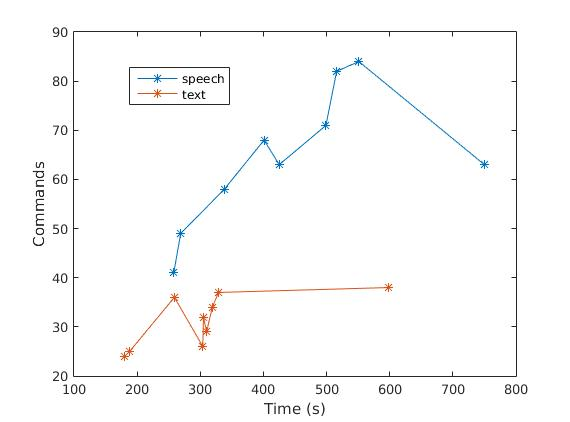
\includegraphics[width=0.8\textwidth]{images/time_cmd.jpg} %width=0.8\textwidth scales the image down to 80 percent of the text-width. Keeps the ratio.
  \caption{Bladiblala}\label{time_cmd}
\end{figure}

\subsection{Timescale}

\begin{table}[h!]
  \centering
  \begin{tabular}{ccc}
    \toprule
    Speech &   & Text\\
    \midrule
    445.22 &   & 310.22\\
    \bottomrule
  \end{tabular}
  \caption{Average Time}\label{avg_time}
\end{table}

\subsection{Commands}
Compare with ideal.

\begin{figure}[h!]
  \centering
  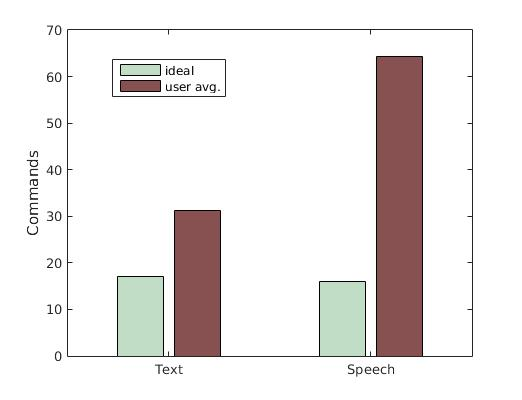
\includegraphics[width=0.8\textwidth]{images/ideal_cmd.jpg}
  \caption{Bladiblala}\label{ideal_cmd}
\end{figure}

This is how you refer to table \ref{avg_cmd} or a graph. You look at the label. See comment in code.

\begin{table}[h!]
  \centering
  \begin{tabular}{ccc}
    \toprule
    Speech &   & Text\\
    \midrule
    64.33 &   & 31.22\\
    \bottomrule
  \end{tabular}
  \caption{Average Commands}\label{avg_cmd} % OMG LOOK HERE!!!
\end{table}

\section{Ease of Use}
Bajskorv

\subsection{English Confidence}

\begin{figure}[p]
  \centering
  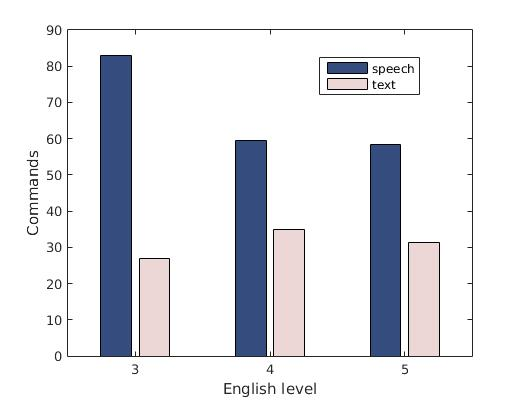
\includegraphics[width=0.8\textwidth]{images/english_cmd.jpg}
  \caption{Bladiblala}\label{eng_cmd}
\end{figure}

\begin{figure}[p]
  \centering
  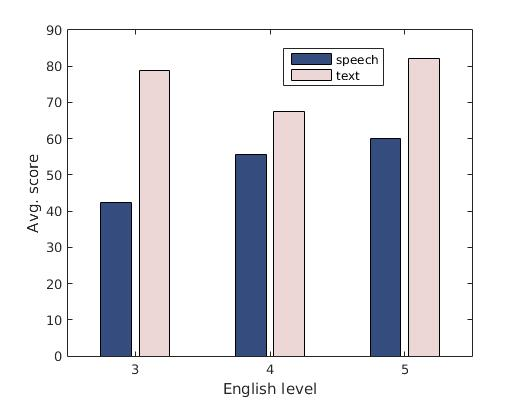
\includegraphics[width=0.8\textwidth]{images/english_score.jpg}
  \caption{Bladiblala}\label{eng_score}
\end{figure}

\begin{figure}[p]
  \centering
  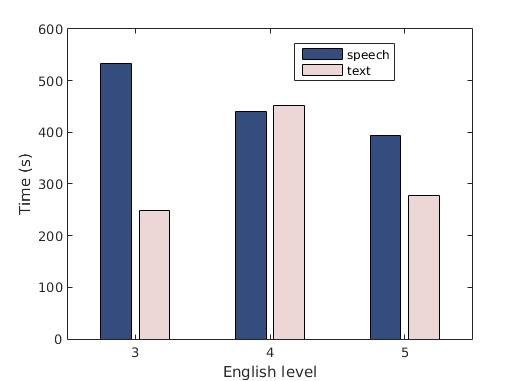
\includegraphics[width=0.8\textwidth]{images/english_time.jpg}
  \caption{Bladiblala}\label{eng_time}
\end{figure}

%\subsection{User Former Experience}

\section{Satisfaction (SUS)}

\begin{figure}[p]
  \centering
  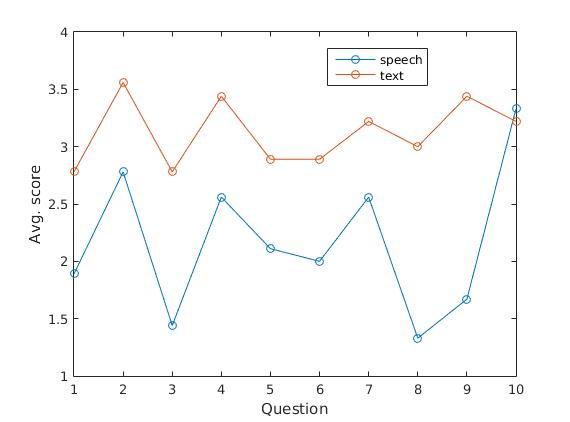
\includegraphics[width=0.8\textwidth]{images/sus.jpg}
  \caption{Bladiblala}\label{sus_table}
\end{figure}

\begin{table}[h!]
  \centering
  \begin{tabular}{ccc}
    \toprule
    Speech &   & Text\\
    \midrule
    54.17 &   & 78.06\\
    \bottomrule
  \end{tabular}
  \caption{Caption for the table.}\label{tot_score}
\end{table}

satisfaction